% title page => wenn es auf englisch sein soll
\begin{titlepage}
\thispagestyle{empty}
\vspace{-1.5cm}
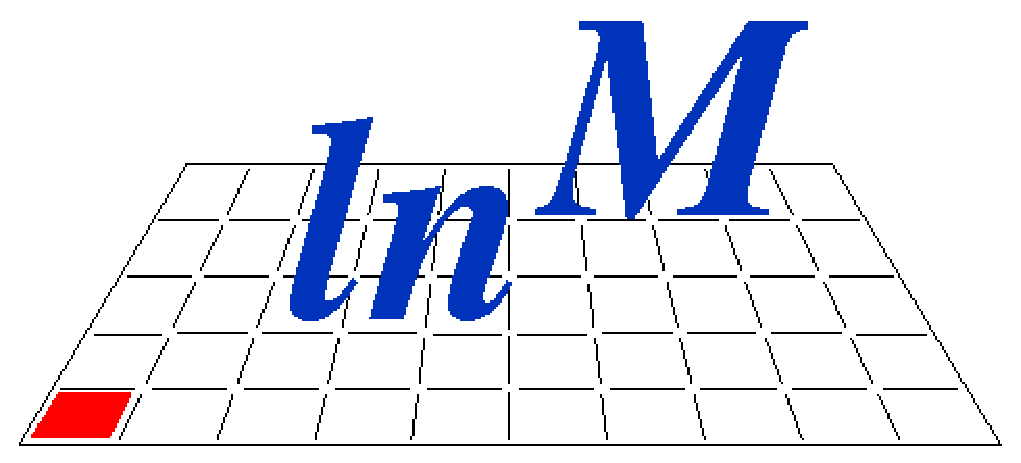
\includegraphics[height=1.5772cm]{./fig/lnm.eps}
\hfill

\includegraphics[height=1.5772cm]{./fig/tum.eps}
\vfill

\begin{center}
\Huge{\thesistitle}
\\
\vspace{0.2cm}
\LARGE{\Author}
\\
\vspace{0.2cm}
\large{\thesistype}
\end{center}
% \vfill
\vspace{0.1cm}
%
% und an diese Stelle kommt ein tolles Bild aus der eigenen Arbeit
\begin{center}

\includegraphics[width=8cm]{fig/nilifem}
\end{center}
%
% \vspace{0.1cm}
\vfill
%
\begin{minipage}[c]{1.0\textwidth}
\centering
{\large \scshape Supervisor:}\\
{\Supervisor}\\ %The Supervisor is specified in the Header file
\texttt{\Mail}\\
\end{minipage}
%
\vspace{1cm}\\
%
\rule{\textwidth}{1pt}
%
\begin{tabular}[t]{l}
Institute for Computational Mechanics
\\
  Prof.\@ Dr.--Ing.\@ W.\ A.\ Wall
\\
Technische Universit\"at M\"unchen
\end{tabular}
\hfill
\begin{tabular}[t]{r}
%   \copyright Lehrstuhl f\"{u}r Numerische Mechanik
\\
Boltzmannstra\ss e 15
\\
85748 Garching b. M\"unchen (Germany)\\
\end{tabular}
\rule{\textwidth}{1pt}


\end{titlepage}